\documentclass[12pt]{article}
\usepackage[T2A]{fontenc}
\usepackage[utf8]{inputenc}
\usepackage[russian]{babel}
\usepackage{graphicx}
\usepackage{amsmath, amssymb}
\usepackage{geometry}
\geometry{a4paper, top=1.5cm, bottom=1.5cm, left=1.5cm, right=1.5cm}
\usepackage{float}
\usepackage{caption}
\usepackage{hyperref}
\usepackage{enumitem}
\usepackage{tikz}
\usepackage{circuitikz} 
\usetikzlibrary{arrows}
\usetikzlibrary{decorations.pathreplacing}
\graphicspath{{pic/}}
\definecolor{water} {rgb} {0.667, 0.855, 1}
\usepackage{pgfplots}
\usepackage{pgfplotstable}
\usetikzlibrary{circuits}
\usetikzlibrary{circuits.ee}
\usetikzlibrary{circuits.ee.IEC}
\usetikzlibrary{circuits.logic.IEC}
\usetikzlibrary{intersections}
% Настройка отступов и шрифтов для академического стиля
% \setlength{\parindent}{1.25cm}
% \linespread{1.5}

% \title{Отчёт по лабораторной работе 4.7.3:\\ \textbf{Поляризация}}
% \author{Фамилия И.О.\\ Группа: \_\_\_\_\_\_\_\_\_\_\_\_\_}
% \date{\today}

\begin{document}

\title{\begin{center}Лабораторная работа №4.7.3:\end{center}
Поляризация}
\author{Струков О. И. \\ Б04-404}
\date{}

\thispagestyle{empty}
\pagenumbering{gobble}
\maketitle
\newpage
\pagenumbering{arabic}

\section*{Теоретическая часть}
\begin{enumerate}
    \item \textbf{Поляризация при отражении (закон Брюстера).} При падении неполяризованного света на границу раздела двух диэлектриков под углом Брюстера $\theta_B$ отражённый луч становится полностью линейно поляризованным. Вектор $\vec{E}$ колебаний параллелен отражающей поверхности («правило иголки»). Угол Брюстера связан с показателем преломления материала соотношением:
    \begin{equation}
        \tan \theta_B = n.
    \end{equation}
    При этом отражённый и преломлённый лучи взаимно перпендикулярны.

    \item \textbf{Двойное лучепреломление и фазовый сдвиг.} В двоякопреломляющих кристаллических пластинках существуют два взаимно перпендикулярных главных направления ($x$ и $y$). Волны, поляризованные вдоль этих осей, распространяются с разными скоростями ($v_x = c/n_x$, $v_y = c/n_y$). При прохождении через пластинку толщиной $d$ между ними возникает разность фаз:
    \begin{equation}
        \Delta \varphi = k d (n_x - n_y) = \frac{2\pi}{\lambda} d (n_x - n_y),
    \end{equation}
    где $\lambda$ -- длина волны в вакууме.

    \item \textbf{Фазовые пластинки.} В зависимости от создаваемой разности хода $\Delta = d|n_x - n_y|$ пластинки классифицируются как:
    \begin{itemize}
        \item $\lambda$-пластинка ($\Delta \varphi = 2\pi$): не изменяет состояние поляризации.
        \item $\lambda/2$-пластинка ($\Delta \varphi = \pi$): поворачивает плоскость поляризации линейного света на угол $2\alpha$ относительно главных осей.
        \item $\lambda/4$-пластинка ($\Delta \varphi = \pi/2$): преобразует линейно поляризованный свет в эллиптически или круговой (при угле $45^\circ$ между $\vec{E}$ и осями пластинки).
    \end{itemize}

    \item \textbf{Интерференция поляризованных лучей.} При помещении двоякопреломляющей пластинки между скрещенными поляроидами когерентные компоненты $E_x$ и $E_y$ проецируются на разрешённое направление анализатора, приобретая дополнительный сдвиг фаз. Результат интерференции зависит от $\lambda$, поэтому при освещении белым светом наблюдается окраска пластинки. Поворот анализатора на $90^\circ$ меняет сдвиг фаз на $\pi$, что инвертирует цвета (позитив $\leftrightarrow$ негатив).

    \item \textbf{Пластинка чувствительного оттенка.} Это $\lambda$-пластинка для зелёного света ($\lambda \approx 560$ нм). При освещении белым светом между скрещенными поляроидами она выглядит лилово-красной (зелёная компонента гасится). При сложении с $\lambda/4$-пластинкой происходит аддитивное или субтрактивное сложение оптических разностей хода, что меняет цвет на зелёно-голубой или оранжево-жёлтый. По изменению цвета определяется направление «быстрой» оси.

    \item \textbf{Определение направления вращения эллипса.} С помощью $\lambda/4$-пластинки, оси которой совмещены с осями эллипса, эллиптически поляризованный свет преобразуется в линейно поляризованный. По квадранту, в котором располагается вектор $\vec{E}$ на выходе, определяется направление вращения электрического вектора (по или против часовой стрелки).
\end{enumerate}

\newpage
\section*{Ход работы}

\subsection*{1. Определение разрешённых направлений поляроидов}
На оптической скамье были размещены источник света, поляроид $P_1$ и чёрное зеркало. Поворачивая поляроид вокруг луча и зеркало вокруг вертикальной оси, методом последовательных приближений была получена минимальная интенсивность отражённого пятна. Затем вместо зеркала был поставлен второй поляроид $P_2$ и повёрнут до максимального затемнения.

\begin{figure}[H]
    \centering
    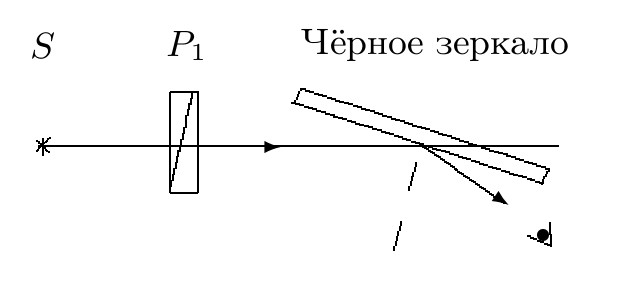
\includegraphics[width=0.6\textwidth]{fig5.jpg}
    \caption{Схема определения разрешённого направления поляроида.}
    \label{fig:setup1}
\end{figure}



Минимум яркости достигается при падении света на зеркало под углом Брюстера и при совпадении плоскости колебаний $\vec{E}$ с плоскостью падения. При скрещивании $P_1$ и $P_2$ интенсивность падает до нуля, что подтверждает их перпендикулярность.

\subsection*{2. Определение показателя преломления эбонита}
Чёрное зеркало было заменено эбонитовым "зеркалом". Был измерен угол поворота (угол Брюстера $\theta_{\text{Б}}$) при минимуме отражённого света. Измерения были повторены с зелёным светофильтром, при этом угол Брюстера остался тем же.

$\theta_{\text{Б}} \approx 57^\circ \implies n = \tg \theta_{\text{Б}} \approx 1,54$, что близко к табличному значению для эбонита $\approx 1,6-1,7$.

\subsection*{3. Исследование поляризации в лучах стопы пластинок}
Стопа стеклянных пластинок была установлена под углом Брюстера. Через поляроид можно было исследовать отражённый и преломлённый лучи.

\begin{figure}[H]
    \centering
    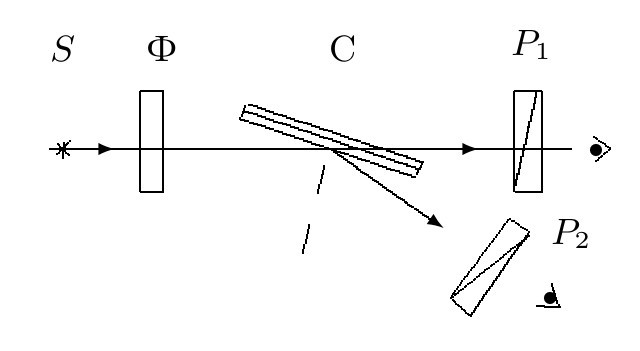
\includegraphics[width=0.6\textwidth]{fig6.jpg}
    \caption{Исследование стопы.}
    \label{fig:setup3}
\end{figure}

В отражённом луче вектор $\vec{E}$ ориентирован перпендикулярно плоскости падения (поляризация полная при угле Брюстера). В преломлённом луче наблюдалась частичная поляризация с преимущественной ориентацией $\vec{E}$ параллельно плоскости падения. При повороте анализатора на $90^\circ$ интенсивность отражённого луча меняется от максимума до минимума.

\subsection*{4. Определение главных направлений двоякопреломляющих пластинок}
Кристаллическая пластинка была помещена между скрещенными поляроидами. При вращении пластинки вокруг луча и можно было наблюдать изменение интенсивности.

\begin{figure}[H]
    \centering
    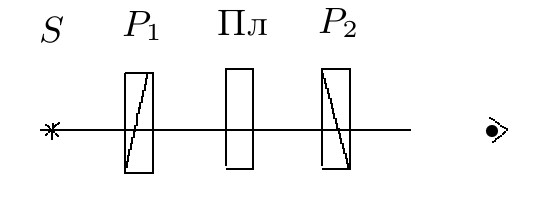
\includegraphics[width=0.6\textwidth]{fig7.jpg}
    \caption{Определение главных направлений в пластинках.}
    \label{fig:setup4}
\end{figure}

Интенсивность обращалась в нуль четыре раза за оборот. Это происходило, когда главные оси кристалла совпадали с разрешёнными направлениями поляроидов. В этих положениях свет не меняет поляризацию и полностью блокируется анализатором.

\subsection*{5. Определение пластинок $\lambda/2$ и $\lambda/4$}
В систему был добавлен зелёный фильтр. Поляризатор $P_1$ был устанавлен горизонтально, оси пластинки -- под углом $45^\circ$ к горизонтали. Свет на выходе можно было анализировать с помощью $P_2$:

\begin{itemize}
    \item Если на выходе свет линейно поляризован и плоскость колебаний повёрнута на $90^\circ$ -- это пластинка $\lambda/2$.
    \item Если поляризация круговая или эллиптическая (интенсивность не меняется при вращении $P_2$) -- это пластинка $\lambda/4$.
\end{itemize}

\subsection*{6. Определение «быстрой» и «медленной» осей в пластинке $\lambda/4$}
Между скрещенными поляроидами была поставлена пластинка чувствительного оттенка (стрелка). Без зелёного фильтра она имеет пурпурный цвет (рис. 5). При добавлении $\lambda/4$-пластинки
в случае совпадения «быстрых» осей разность хода суммируется ($5\lambda/4$), что соответствует гашению более длинных волн, поэтому цвет становится голубым (рис. 6). При перпендикулярных осях разность хода вычитается ($3\lambda/4$), гасятся короткие волны, и цвет жёлтый (рис. 7). Таким образом, при голубом цвете быстрые оси совпадают.

\begin{figure}[H]
    \centering
    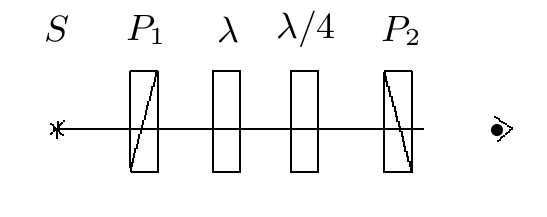
\includegraphics[width=0.6\textwidth]{fig8.jpg}
    \caption{Определение направлений скорости.}
\end{figure}

\begin{figure}[H]
    \centering
    
\includegraphics[width=0.5\textwidth]{2.jpg}
    \caption{Пластинка без фильтра.}
\end{figure}

\begin{figure}[H]
    \centering
    \begin{minipage}{0.45\textwidth}
        \centering
        
\includegraphics[width=\textwidth]{3.jpg}
        \caption{Изменение цвета при совмещении осей.}
    \end{minipage}\hfill
    \begin{minipage}{0.45\textwidth}
        \centering
        
\includegraphics[width=\textwidth]{1.jpg}
        \caption{Изменение цвета при скрещивании осей.}
    \end{minipage}
\end{figure}

% \begin{figure}[H]
%     \centering
%     
\includegraphics[width=0.7\textwidth]{3.jpg}
%     \caption{Изменение цвета при совмещении осей.}
% \end{figure}

% \begin{figure}[H]
%     \centering
%     
\includegraphics[width=0.7\textwidth]{1.jpg}
%     \caption{Изменение цвета при скрещивании осей.}
% \end{figure}

\subsection*{7. Интерференция поляризованных лучей}
Для исследования интерференции была использована мозаичная слюдяная пластинка (полоски с $\lambda/4$, $\lambda/2$, $3\lambda/4$) между скрещенными поляроидами. В результате эксперимента определено:
\begin{itemize}
    \item При вращении мозаики цвет не меняется, меняется только интенсивность. Это связано с тем, что $\Delta \varphi$ зависит только от толщины и $\lambda$, а не от угла поворота.
    \item При повороте второго поляроида на $90^\circ$ волны $E_1$ и $E_2$ приобретают дополнительный сдвиг $\pi$. Цвет каждого квадратика меняется. Интенсивность изменяется только у центрального, не имеющего пластинок из слюды.
\end{itemize}

\begin{figure}[H]
    \centering
    \begin{minipage}{0.45\textwidth}
        \centering
        
\includegraphics[width=\textwidth]{5.jpg}
        \caption{Интерференционная картина в мозаичной пластинке.}
    \end{minipage}\hfill
    \begin{minipage}{0.45\textwidth}
        \centering
        
\includegraphics[width=\textwidth]{4.jpg}
        \caption{Интерференционная картина после поворота второго поляризатора.}
    \end{minipage}
\end{figure}


\subsection*{8. Определение направления вращения светового вектора}

\begin{enumerate}
    \item Было построено качественное изображение эллипса поляризации для световой волны, прошедшей через пластинку $\lambda/4$ (рис. 10). Главной оси $x$ соответствует наибольшая скорость распространения. Справа изображены временные зависимости проекций вектора напряжённости поля $x(t)$ и $y(t)$, демонстрирующие фазовый сдвиг $\Delta\varphi = \pi/2$.
    
    \item В оптическую схему вновь был внесён зелёный светофильтр, после которого между скрещенными поляризаторами размещена пластинка $\lambda/4$ с соседней установки.
    
    \item Для формирования эллиптически поляризованного излучения разрешённая плоскость первого поляроида была ориентирована под углом около $15^\circ$ к горизонтали, что обеспечивало расположение вектора $\vec{E}$ падающего пучка в первом квадранте системы координат. Разрешённое направление второго поляроида было зафиксировано в вертикальном положении. При повороте кристаллической пластинки было получено минимальное значение интенсивности света, прошедшего через анализатор. Последующее вращение анализатора подтвердило наличие эллиптической поляризации. В результате был сформирован эллипс с вертикально ориентированной малой осью.
    
    % \item Чтобы выявить направление вращения электрического вектора, в промежуток между поляризаторами была введена дополнительная четвертьволновая пластинка, «быстрая» ось которой была ориентирована горизонтально и совмещена с осями исследуемого эллипса. Проходя через последовательность двух $\lambda/4$-пластинок, волна на выходе приобретает линейную поляризацию. Характер интерференции зависит от знака начального сдвига фаз: если направления вращения эллипсов в первой и второй пластинках противоположны, происходит взаимная компенсация разности хода, и результирующий вектор $\vec{E}$ сохраняется в I и III квадрантах. При совпадении направлений вращения фазы суммируются, что приводит к переходу вектора во II и IV квадранты. Сопоставив экспериментальный результат с теоретическим анализом, проведённым в пункте 1, однозначно установили характер вращения светового вектора в исходной волне.
\end{enumerate}



% Был нарисован эллипс поляризации для вектора $\vec{E}$, вышедшего из пластинки $\lambda/4$ , где большей скорости соответствует ось $x$, а также две вышедших из пластинки синусоиды: $x(t)$ и $y(t)$ со сдвигом фаз в четверть периода (рис. 10). Проанализировали графики и определили направление вращения электрического вектора в эллиптически поляризованной волне.

% б) Получаем эллиптически поляризованный свет, установив $P_1$ под $10-20^\circ$, а $P_2$ вертикально. 
% в) Вставляем $\lambda/4$ с горизонтальной быстрой осью и определяем квадрант выхода.

		\begin{figure}[H]
		    \centering
		    \begin{tikzpicture}[>=latex', scale=0.7]
		        \draw[->] (-3,0) -- (3, 0)node[below]{$x$};
		        \draw[->] (0,-2) -- (0, 2)node[left]{$y$};
		        \draw (0,0) ellipse (2.2 and 1.4);
		        \draw[->] (2.2, 0) -- (2.2, 0.001);
		        \draw[->] (-2.2, 0) -- (-2.2, -0.001);
		        \draw[->] (0, 1.4) -- (-0.001, 1.4);
		        \draw[->] (0, -1.4) -- (0.001, -1.4);
		        \begin{scope}[xshift=280]
		        \clip (-4,-3) rectangle (4.5, 3);
		        \draw (0, 0) sin (-1.57,-1.3);
		        \draw (0, 0) sin (1.57,1.3);
		        \draw (3.14, 0) sin (1.57, 1.3);
		        \draw (-3.14, 0) sin (-1.57, -1.3);
		        \draw (-4.71, 1.3) cos (-3.14, 0);
		        \draw (3.14, 0) sin (4.71, -1.3);
		        \begin{scope}[xshift=0.785cm]
		        \draw (0, 0) sin (-1.57,-1.3);
		        \draw (0, 0) sin (1.57,1.3);
		        \draw (3.14, 0) sin (1.57, 1.3);
		        \draw (-3.14, 0) sin (-1.57, -1.3);
		        \draw (-4.71, 1.3) cos (-3.14, 0);
		        \draw (3.14, 0) sin (4.71, -1.3);
		        \draw (-3.5, 0.8) --++ (0.5, 0.5) node[right]{$y(t)$};
		        \draw (-3.5, -0.8) --++ (-0.5, -0.5) node[below]{$x(t)$};
		        \end{scope}
		        \draw[->] (-4,0) -- (4.5, 0)node[above left]{$t$};
		        \draw[->] (0,-2) -- (0, 2)node[left]{$E$};
		        \draw (0, -0.1) -- (0,0.1) node[anchor=south east,fill=white] {0};
		        \draw (0.785, 0.1) -- (0.785, -0.1) node[anchor=north west,fill=white] {$\frac{T}{4}$};
		        \draw (3.14, 0.1) -- (3.14, -0.1) node[anchor=north east,fill=white] {$T$};
		        \end{scope}
		    \end{tikzpicture}
		    \caption{Эллипс поляризации и графики компонент.}
		\end{figure}



% При компенсации разности фаз $\lambda/4$-пластинкой свет становится линейно поляризованным. Если вектор $\vec{E}$ остался в 1-м и 3-м квадрантах $\rightarrow$ эллипсы вращались в \textbf{разные} стороны. Если перешёл во 2-й и 4-й $\rightarrow$ вращение в \textbf{одну} сторону. 

\section*{Вывод}
В ходе выполнения работы были экспериментально изучены основные методы получения и анализа поляризованного света. С помощью чёрного зеркала определены разрешённые направления поляроидов и измерен угол Брюстера для эбонита, что позволило рассчитать его показатель преломления $n \approx 1,54$. Исследована поляризация отражённого и преломлённого света стопой пластинок, подтверждено правило Брюстера. 

Были идентифицированы двоякопреломляющие пластинки $\lambda/2$ и $\lambda/4$ по изменению состояния поляризации. С использованием пластинки чувствительного оттенка были определены «быстрая» и «медленная» оси в $\lambda/4$-пластинке на основе эффекта аддитивного и субтрактивного сложения оптических разностей хода.
Исследована интерференция поляризованных лучей, объяснена смена цветов при повороте анализатора. Методом компенсации разности фаз определено направление вращения электрического вектора в эллиптически поляризованной волне. Все полученные результаты согласуются с теоретическими ожиданиями.

\end{document}
